% author Dinupa Nawarathne
% email dinupa3@gmail.com
% date 09-29-2022

\documentclass[12pt, xcolor={dvipsnames}, aspectratio = 169]{beamer}

%
% packages
%
\usepackage{graphicx}
\usepackage{amsmath}
\usepackage{hyperref}
\usepackage[absolute,overlay]{textpos}
\usepackage{mathrsfs}
\usepackage[font=tiny]{caption}

%
% customization
%
\mode<presentation>
{
% custom colors
\definecolor{nmsured}{RGB}{137,18,22}
% custom fonts
\usefonttheme{serif}
\setbeamercolor{title}{bg=White,fg=nmsured}
\setbeamercolor{frametitle}{bg=White,fg=nmsured}
\setbeamercolor{section number projected}{bg=nmsured,fg=White}
\setbeamercolor{subsection number projected}{bg=nmsured,fg=White}
\setbeamertemplate{items}{\color{nmsured}$\blacksquare$}
\setbeamertemplate{section in toc}[square]
\setbeamertemplate{subsection in toc}[square]
\setbeamertemplate{footline}[frame number]
\setbeamertemplate{caption}[numbered]
\setbeamerfont{footnote}{size=\tiny}
\setbeamercovered{invisible}
}

%
% title, author, date
%
\title{HotEncoding and Tagging of the Single $\mu$ Tracks}

\author{Dinupa}

\date{NMSU Update
\\ October 11, 2022 }

\begin{document}

% make title page
\begin{frame}
    \maketitle
\end{frame}


% 1st slide
\begin{frame}{MLP Neural Network}
\begin{textblock}{14.0}(0.1, 2.0)
    \begin{figure}
        \centering
        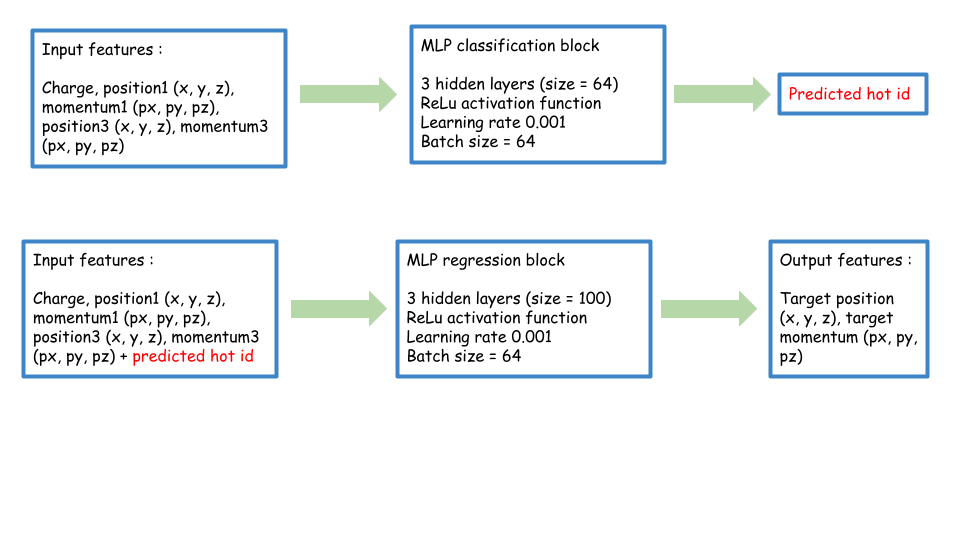
\includegraphics[width=14.0cm]{../imgs/flow-chart.png}
    \end{figure}
\end{textblock}
\end{frame}


% 2nd slide
\begin{frame}[fragile]{One Hot Encoding}

\begin{textblock}{7.0}(0.5, 2.0)

    \begin{itemize}
        \item We used the \verb|OneHotEncoder| class in \verb|sklearn|.
        \item Encode categorical features as a one-hot numeric array.
        \item By default, the encoder derives the categories based on the unique values in each feature.
    \end{itemize}

\end{textblock}

\begin{textblock}{7.0}(7.0, 2.0)
    \begin{verbatim}
    position          | label      | int
    ------------------------------------
    -800. < z < -305. | collimeter | 0
    -305. < z < -295. | target     | 1
    -295. < z < -1.   | other      | 2
    -1. < z < 500.    | beam dump  | 3
    \end{verbatim}
\end{textblock}

\begin{textblock}{7.0}(0.2, 9.0)
    \begin{verbatim}
               | collimeter | target | other | beam dump |
    ------------------------------------------------------
    collimeter | 1          | 0      | 0     | 0         |
    target     | 0          | 1      | 0     | 0         |
    other      | 0          | 0      | 1     | 0         |
    beam dump  | 0          | 0      | 0     | 1         |
    ------------------------------------------------------
    \end{verbatim}
\end{textblock}

\end{frame}


% 3rd slid
\begin{frame}[fragile]{Tagging Task}
    \begin{textblock}{8.0}(0.2, 1.0)
        \begin{figure}
            \centering
            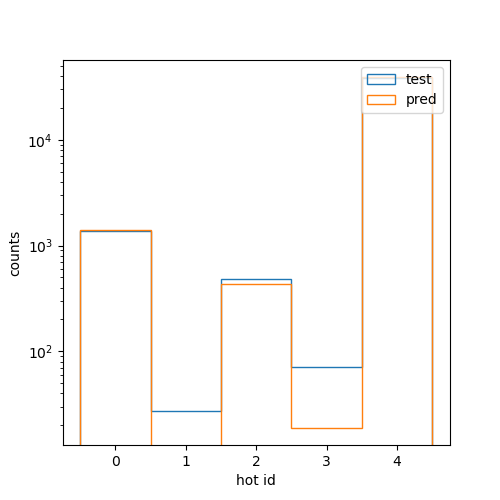
\includegraphics[width=8.0cm]{../imgs/cls-hot-id.png}
        \end{figure}
    \end{textblock}
    
    \begin{textblock}{7.0}(8.0, 2.0)
    
    \begin{itemize}
        \item Classification layer almost predict bins except for bin with \verb|hot_id = 2|, with 
        \verb|classification score = 0.9895|
    \end{itemize}
    
    \end{textblock}
    
\end{frame}

% 4th slide
\begin{frame}

\begin{textblock}{8.0}(0.2, 0.2)
    \begin{figure}
        \centering
        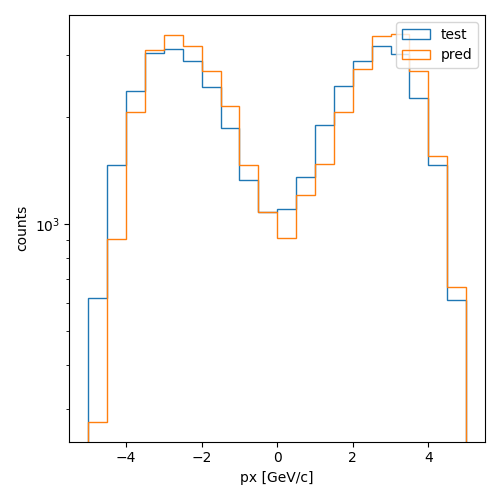
\includegraphics[width=8.0cm]{../imgs/cls-vpx.png}
    \end{figure}
\end{textblock}

\begin{textblock}{8.0}(8.0, 0.2)
    \begin{figure}
        \centering
        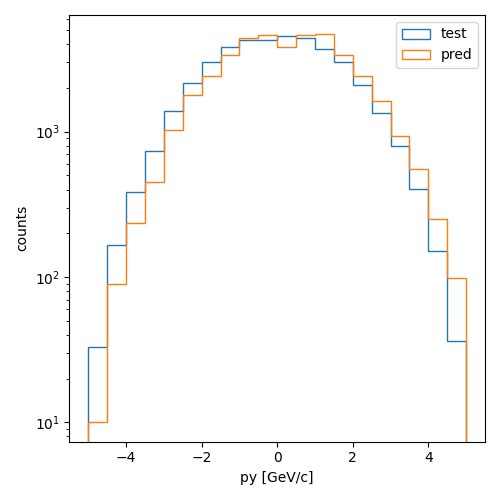
\includegraphics[width=8.0cm]{../imgs/cls-vpy.png}
    \end{figure}
\end{textblock}

\end{frame}

% 5th slide
\begin{frame}[fragile]

\begin{textblock}{8.0}(0.2, 0.2)
    \begin{figure}
        \centering
        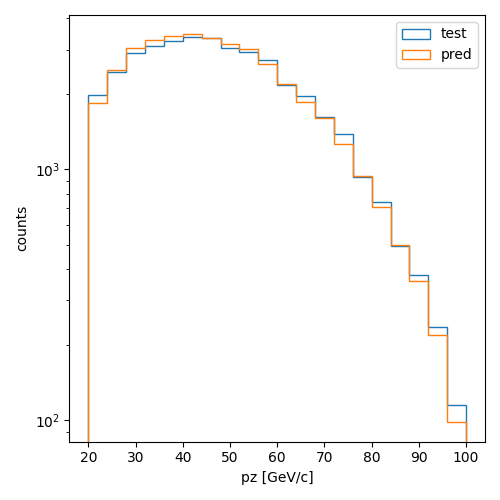
\includegraphics[width=8.0cm]{../imgs/cls-vpz.png}
    \end{figure}
\end{textblock}

\begin{textblock}{8.0}(8.0, 2.0)
    \begin{itemize}
        \item \verb|vpx, vpy, vpz| has a good prediction.
    \end{itemize}
\end{textblock}

\end{frame}

% 6th slide
\begin{frame}[fragile]

\begin{textblock}{8.0}(0.2, 0.2)
    \begin{figure}
        \centering
        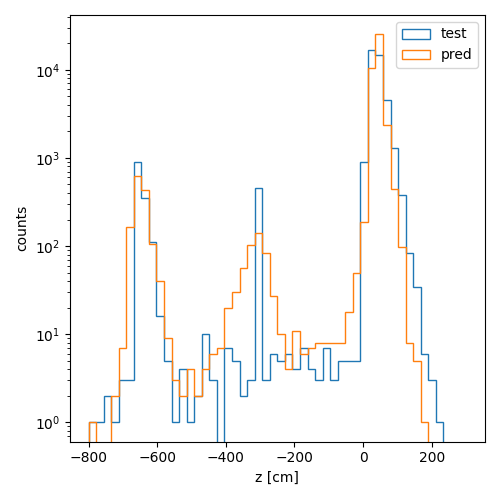
\includegraphics[width=8.0cm]{../imgs/cls-vtz.png}
    \end{figure}
\end{textblock}

\begin{textblock}{8.0}(8.0, 2.0)
    \begin{itemize}
        \item With Tagging we can increase the \verb|vtz| prediction.
    \end{itemize}
\end{textblock}

\end{frame}

% 7th slide
\begin{frame}

\begin{textblock}{8.0}(0.2, 0.2)
    \begin{figure}
        \centering
        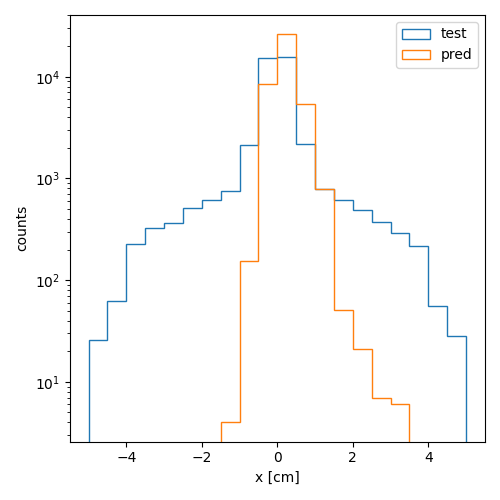
\includegraphics[width=8.0cm]{../imgs/cls-vtx.png}
    \end{figure}
\end{textblock}

\begin{textblock}{8.0}(8.0, 0.2)
    \begin{figure}
        \centering
        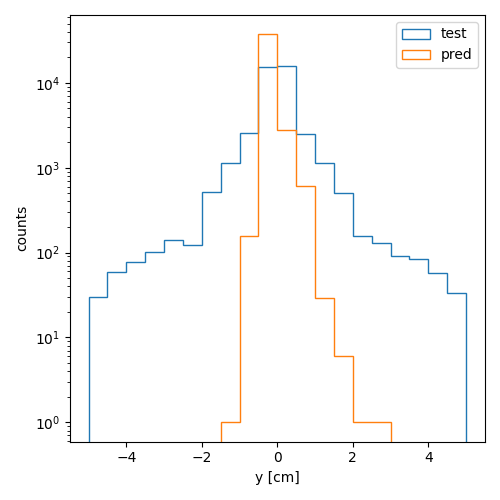
\includegraphics[width=8.0cm]{../imgs/cls-vty.png}
    \end{figure}
\end{textblock}

\end{frame}

% 8th slide
\begin{frame}[fragile]{Summary}

\begin{textblock}{14.0}(0.5, 2.0)
    \begin{itemize}
        \item With tagging we can get a better z-vertex prediction ?
        \item This module was build using \verb|MLPClassifier, MLPRegressor| classes in \verb|sklearn| library. Therefore, saving the trained module and getting the loss values after ephocs is not straight formward.
        \item Since no GPU support is not included it is hard to scale up the module. Better to build the neural network with \verb|pytorch|. (working on this)
    \end{itemize}
\end{textblock}

\end{frame}


\end{document}
